
\begin{figure}[htp]
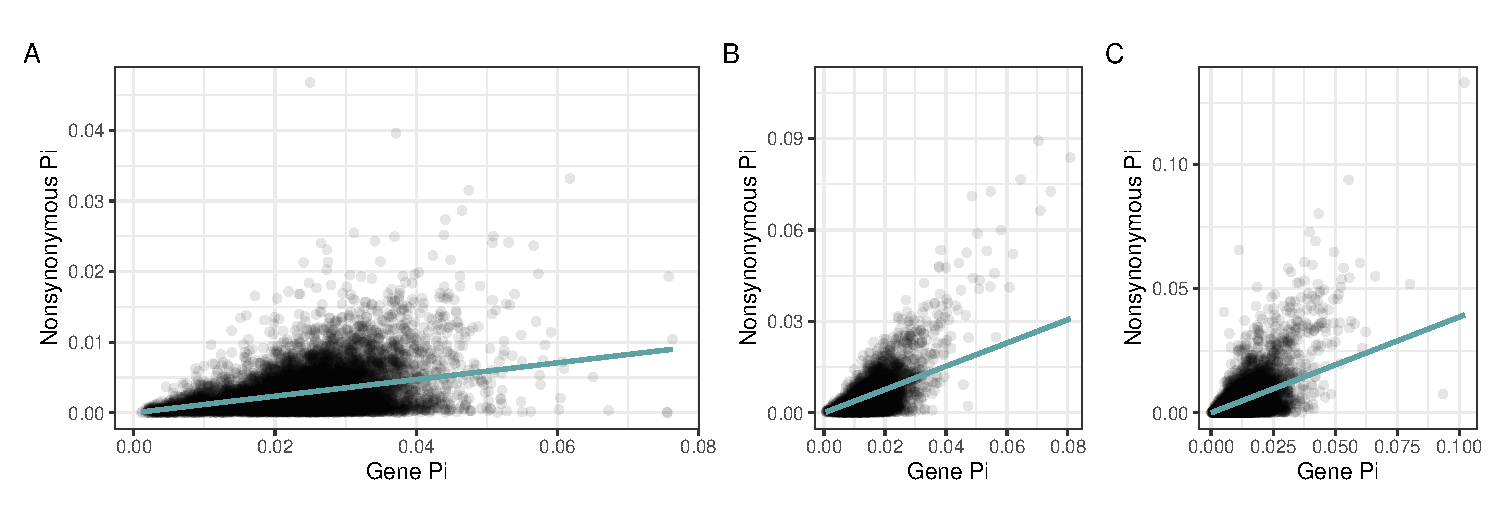
\includegraphics[width=\linewidth]{figures/ns_pi_vs_gene_pi.pdf}
\centering
\caption{Relationship between $\pi_{N}$ and $\pi_G$ in \textit{An. gambiae} (A), \textit{funestus} (B), and \textit{minimus} (C).}
\label{fig:pilm}
\end{figure}

\begin{figure}[htp]
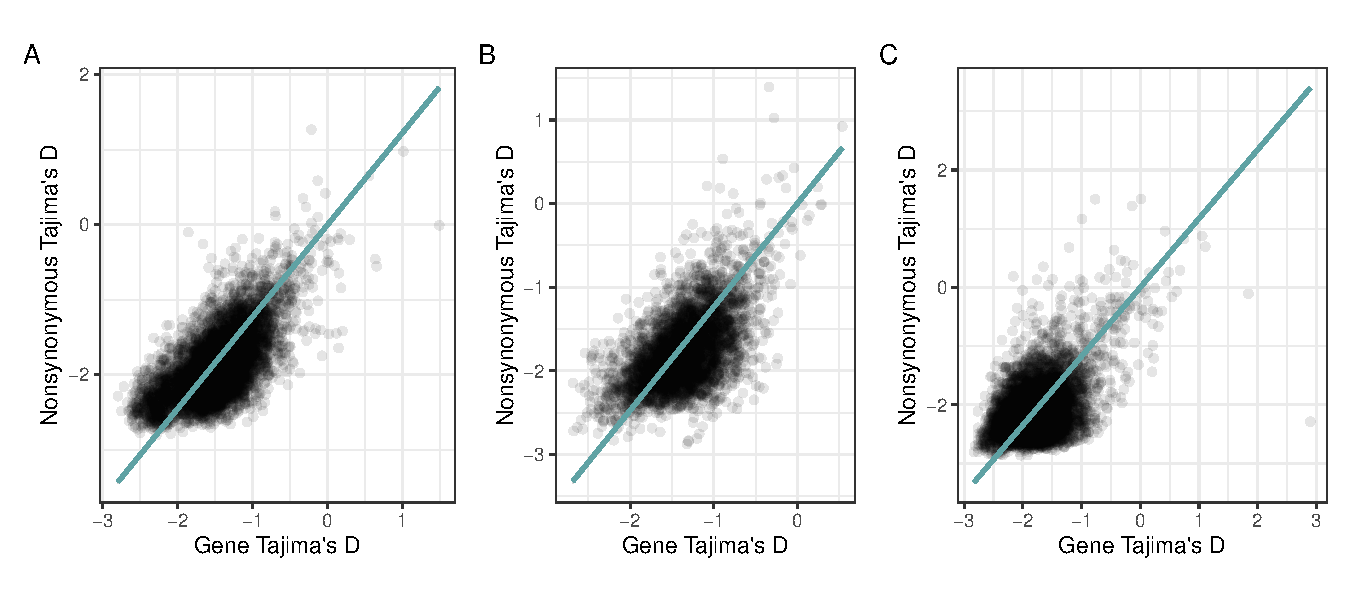
\includegraphics[width=\linewidth]{figures/ns_d_vs_gene_d.pdf}
\centering
\caption{Relationship between $D_N$ and $D_G$ in \textit{An. gambiae} (A), \textit{funestus} (B), and \textit{minimus} (C).}
\label{fig:dlm}
\end{figure}

\begin{figure}[htp]
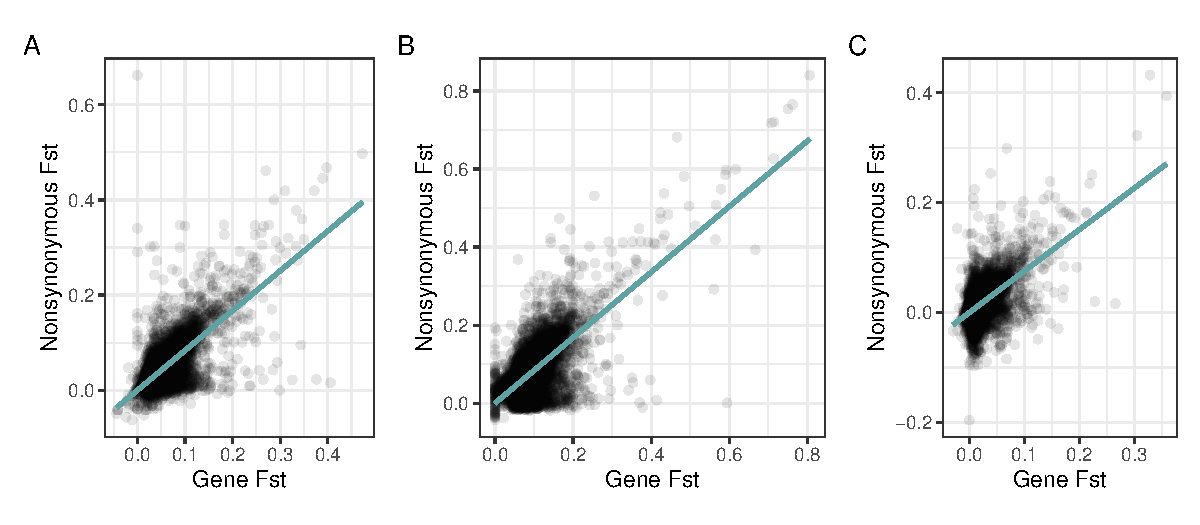
\includegraphics[width=\linewidth]{figures/ns_fst_vs_gene_fst.pdf}
\centering
\caption{Relationship between $F_{ST_{NS}}$ and $F_{G_{NS}}$ in \textit{An. gambiae} (A), \textit{funestus} (B), and \textit{minimus} (C).}
\label{fig:fstlm}
\end{figure}

\section{GO enrichments for \texorpdfstring{$\pi_{N}$}{nonsynonymous pi}}

\subsection{\textit{An. gambiae}}

\begin{table}[H]
    \centering
    \begin{tabular}{clc}
        \toprule
        \textbf{GO ID}& \textbf{Term} & \textbf{p value}\\
        \midrule
        GO:0007608 & sensory perception of smell & 0.00024 \\ 
        GO:0006508 & proteolysis & 0.00793 \\ 
        GO:0006310 & DNA recombination & 0.01196 \\ 
        GO:0006259 & DNA metabolic process & 0.01383 \\ 
        GO:0006281 & DNA repair & 0.02287 \\ 
        GO:0006284 & base-excision repair & 0.02768 \\ 
        GO:0006974 & DNA damage response & 0.02866 \\ 
        GO:0030150 & protein import into mitochondrial matrix & 0.03312 \\ 
        GO:0006029 & proteoglycan metabolic process & 0.03854 \\ 
        GO:0030166 & proteoglycan biosynthetic process & 0.03854 \\ 
        GO:0170036 & import into the mitochondrion & 0.03854 \\ 
        GO:0006260 & DNA replication & 0.04256 \\ 
        GO:0033554 & cellular response to stress & 0.04316 \\ 
        GO:0000724 & double-strand break repair via homologous recombination& 0.04393 \\ 
        GO:0000725 & recombinational repair & 0.04393 \\ 
        GO:0016073 & snRNA metabolic process & 0.04393 \\ 
        GO:0016180 & snRNA processing & 0.04393 \\ \bottomrule
    \end{tabular}
        \caption{Significant Biological Process GO term enrichments for \textit{An. gambiae} $\pi_{N}$ outliers.}
    \label{gambGOpi}
\end{table}

\subsection{An. funestus}

\begin{table}[H]
    \centering
    \begin{tabular}{clc}
        \toprule
        \textbf{GO ID} & \textbf{Term} & \textbf{p value} \\
        \midrule
        GO:0007281 & germ cell development & 0.00066 \\ 
        GO:0022412 & cellular process involved in reproduction & 0.00066 \\ 
        GO:0003006 & developmental process involved in reproduction & 0.00085 \\ 
        GO:0007276 & gamete generation & 0.00106 \\ 
        GO:0006325 & chromatin organization & 0.00207 \\ 
        GO:0007156 & homophilic cell adhesion via plasma membrane & 0.00727 \\ 
        GO:0098742 & cell-cell adhesion via plasma-membrane adhesion & 0.00782 \\ 
        GO:0098609 & cell-cell adhesion & 0.00840\\ 
        GO:0006814 & sodium ion transport & 0.01294 \\ 
        GO:0048468 & cell development & 0.01515 \\ 
        GO:0030154 & cell differentiation & 0.03040\\ 
        GO:0048869 & cellular developmental process & 0.03040\\ 
        GO:0007155 & cell adhesion & 0.04726 \\ \bottomrule
    \end{tabular}
        \caption{Significant Biological Process GO term enrichments for \textit{An. funestus} $\pi_{N}$ outliers.}
    \label{afunGOpi}
\end{table}

\subsection{An. minimus}

\begin{table}[H]
    \centering
\begin{tabular}{clc}
        \toprule
        \textbf{GO ID} & \textbf{Term} & \textbf{p value} \\
        \midrule
        GO:0051336 & regulation of hydrolase activity & 0.00011 \\ 
        GO:0051246 & regulation of protein metabolic process & 0.00016 \\ 
        GO:0050790 & regulation of catalytic activity & 0.00060\\ 
        GO:0065009 & regulation of molecular function & 0.00093 \\ 
        GO:0000723 & telomere maintenance & 0.02931 \\ 
        GO:0032200 & telomere organization & 0.02931 \\ \bottomrule
    \end{tabular}
        \caption{Significant Biological Process GO term enrichments for \textit{An. minimus} $\pi_{N}$ outliers.}
    \label{aminGOpi}
\end{table}

\section{GO enrichments for \texorpdfstring{Tajima's $D_N$}{nonsynonymous Tajima's $D$}}

\subsection{\textit{An. gambiae}}
\begin{table}[H]
    \centering
    \begin{tabular}{clc}
        \toprule
        \textbf{GO ID}& \textbf{Term} & \textbf{p value}\\
        \midrule
        GO:0006508 & proteolysis & 0.0014 \\ 
        GO:0006749 & glutathione metabolic process & 0.0054 \\ 
        GO:0006575 & modified amino acid metabolic process & 0.0092 \\ 
        GO:0043603 & amide metabolic process & 0.0182 \\ 
        GO:0006790 & sulfur compound metabolic process & 0.0197 \\ 
        GO:0006098 & pentose-phosphate shunt & 0.0229 \\ 
        GO:0006740 & NADPH regeneration & 0.0229 \\ 
        GO:0051156 & glucose 6-phosphate metabolic process & 0.0257 \\ 
        GO:0006739 & NADP metabolic process & 0.0285 \\ 
        GO:0007608 & sensory perception of smell & 0.0353 \\ \bottomrule
    \end{tabular}

    \caption{Significant Biological Process GO term enrichments for \textit{An. gambiae} $D_N$ outliers.}
    \label{gambGOd}
    
\end{table}

\subsection{\textit{An. funestus}}
\begin{table}[H]
    \centering
    \begin{tabular}{clc}
        \toprule
        \textbf{GO ID}& \textbf{Term} & \textbf{p value}\\
        \midrule
        GO:0030301 & cholesterol transport & 0.027 \\ 
        GO:0032367 & intracellular cholesterol transport & 0.027 \\ 
        GO:0032365 & intracellular lipid transport & 0.030\\ 
        GO:0032366 & intracellular sterol transport & 0.030\\ 
        GO:0006096 & glycolytic process & 0.036 \\ 
        GO:0006195 & purine nucleotide catabolic process & 0.036 \\ 
        GO:0009134 & nucleoside diphosphate catabolic process & 0.036 \\ 
        GO:0009137 & purine nucleoside diphosphate catabolic process& 0.036 \\ 
        GO:0009154 & purine ribonucleotide catabolic process & 0.036 \\ 
        GO:0009181 & purine ribonucleoside diphosphate catabolic process& 0.036 \\ 
        GO:0009191 & ribonucleoside diphosphate catabolic process& 0.036 \\ 
        GO:0009261 & ribonucleotide catabolic process & 0.036 \\ 
        GO:0015850 & organic hydroxy compound transport & 0.036 \\ 
        GO:0015918 & sterol transport & 0.036 \\ 
        GO:0019364 & pyridine nucleotide catabolic process & 0.036 \\ 
        GO:0046032 & ADP catabolic process & 0.036 \\ 
        GO:0072526 & pyridine-containing compound catabolic process& 0.036 \\ 
        GO:0009135 & purine nucleoside diphosphate metabolic process& 0.039 \\ 
        GO:0009179 & purine ribonucleoside diphosphate metabolic process& 0.039 \\ 
        GO:0009185 & ribonucleoside diphosphate metabolic process& 0.039 \\ 
        GO:0046031 & ADP metabolic process & 0.039 \\ 
        GO:0009132 & nucleoside diphosphate metabolic process & 0.042 \\ 
        GO:0016052 & carbohydrate catabolic process & 0.048 \\ \bottomrule
    \end{tabular}

    \caption{Significant Biological Process GO term enrichments for \textit{An. funestus} $D_N$ outliers.}
    \label{afunGOd}
    
\end{table}

\subsection{\textit{An. minimus}}
\begin{table}[htbp]
    \centering
    \begin{tabular}{clc}
        \toprule
        \textbf{GO ID}& \textbf{Term} & \textbf{p value}\\
        \midrule
        GO:0050790 & regulation of catalytic activity & 0.00044 \\ 
        GO:0051246 & regulation of protein metabolic process & 0.00112 \\ 
        GO:0043462 & regulation of ATP-dependent activity & 0.0408 \\ 
        GO:0007606 & sensory perception of chemical stimulus & 0.0498 \\ \bottomrule
    \end{tabular}

    \caption{Significant Biological Process GO term enrichments for \textit{An. minimus} $D_N$ outliers.}
    \label{aminGOd}
    
\end{table}

\section{\textit{An. gambiae} and \textit{funestus} $F_{ST_{NS}}$ correlation}

\begin{figure}[htp]
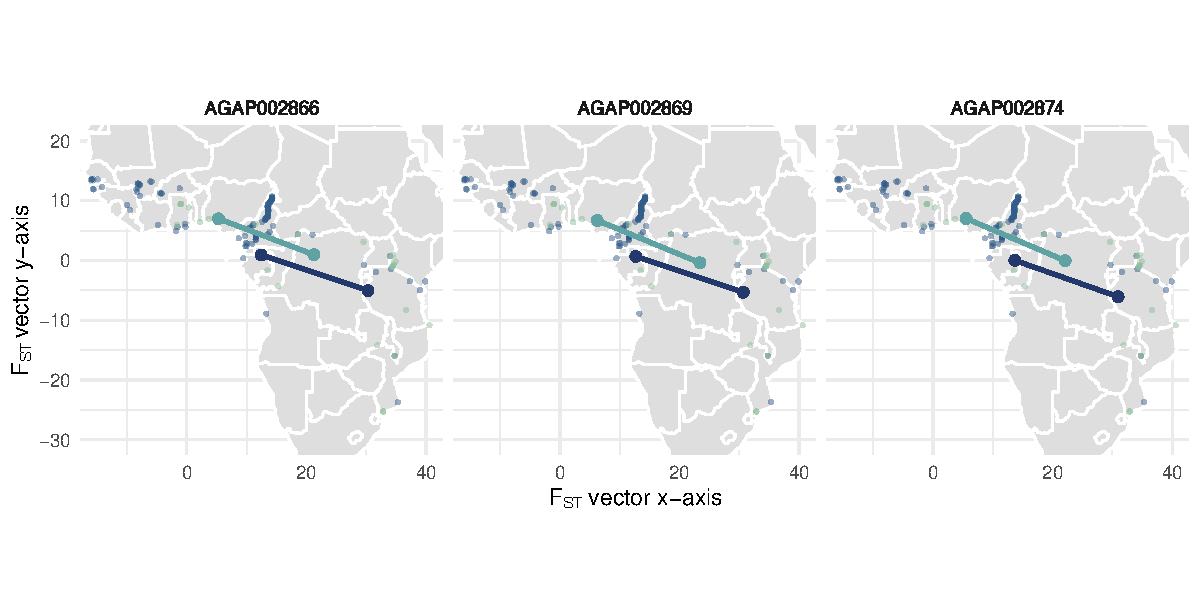
\includegraphics[width=\linewidth]{figures/gamb_afun_fst_correlation_map.pdf}
\centering
\caption{Significantly correlated $F_{ST_{NS}}$ vectors for three \textit{An. gambiae} (dark blue) and \textit{funestus} (light blue) orthologs. Vectors for each species are depicted via a line connecting two points; sampling locations are depicted in points.}
\label{fig:fst_corr}
\end{figure}

\begin{figure}[htp]
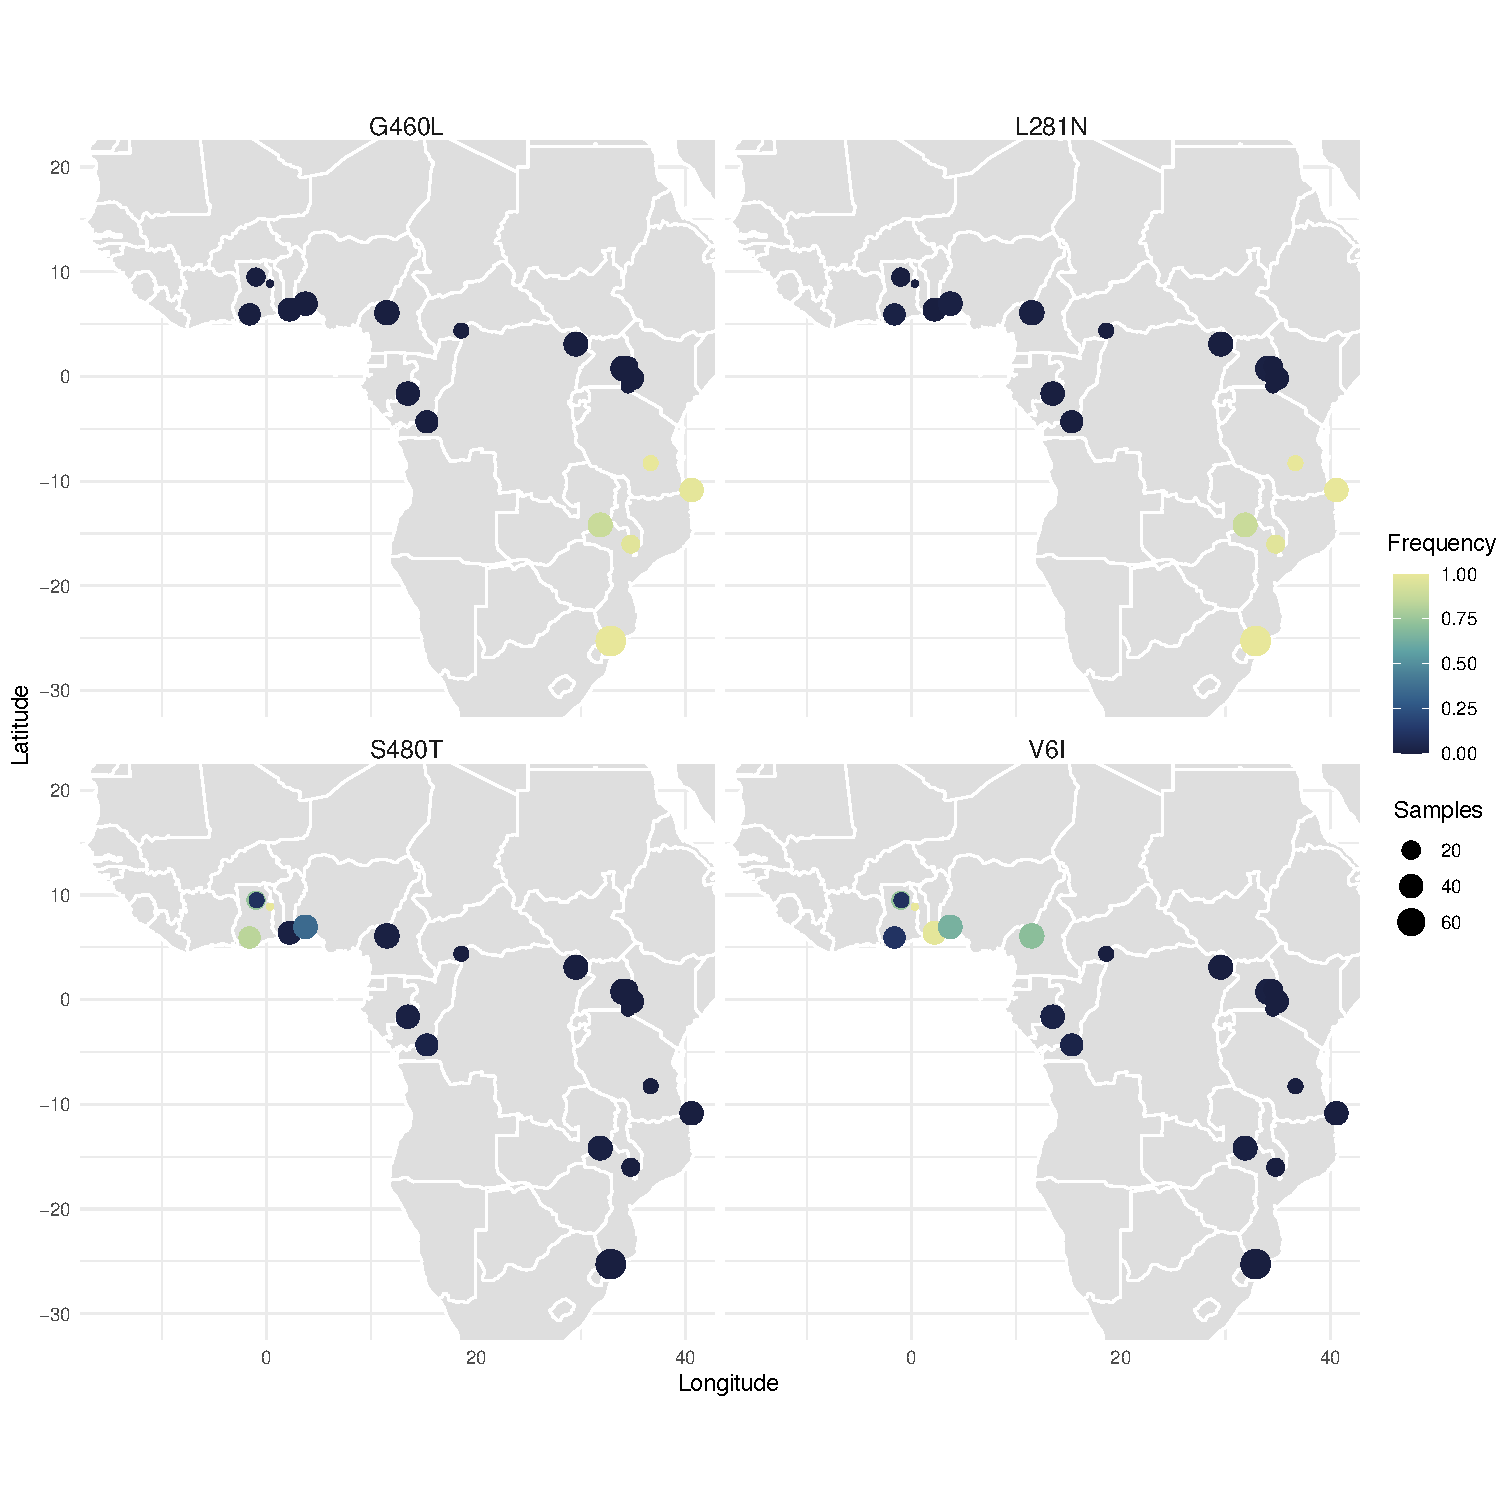
\includegraphics[width=\linewidth]{figures/AFUN2_013651_mutations.pdf}
\centering
\caption{Restricted spatial distribution of high-frequency nonsynonymous alleles in \textit{An. funestus} gene AFUN2\_013651.}
\label{fig:afun_cyp}
\end{figure}
